%-------------------------------------------------------------------------------
\section{Strategy for the $\Htautau$ search}
\label{sec:strategy_Htautau}
%-------------------------------------------------------------------------------

The analysis strategy adopted by the $\Htautau$ search follows closely that developed in Ref.~\cite{Chen:2015nta} and is summarised in this section.

\subsection{Event categorisation and kinematic reconstruction}
\label{sec:htautau_reco_cat}

In the $\Htautau$ search, the $\ttbar \to WbHq$ signal being probed is characterised by the presence of $\tau$-leptons from the decay of 
the Higgs boson and at least four jets, only one of which originates from a $b$-quark.
%In the $\Htautau$ search, the final state signature of interest is characterised by the presence of two $\tau$-leptons from the
%decay of the Higgs boson as well as a light-quark jet, the latter two originating from the decay of one of the top quarks. 
If one of the $\tau$-leptons decays leptonically, an isolated electron or muon and significant $\met$ is also expected.
%The other top quark decays into a $W$ boson and a $b$-quark, with the $W$ boson in turn decaying hadronically, resulting in 
%three additional jets. Therefore, at least four jets are typically expected in signal events.
However, in a significant fraction of the events the trailing jet from the $W$-boson decay fails the minimum $\pt$ requirement of $30~\gev$,
resulting in signal events with only three jets reconstructed.
In order to optimise the sensitivity of the search, the selected events are categorised into four SRs depending 
on the number of $\taulep$ and $\tauhad$ candidates, and on the number of jets:
($\lephad$, 3j), ($\lephad$, $\geq$4j), ($\hadhad$, 3j), and ($\hadhad$, $\geq$4j). 

This event categorisation is primarily motivated by the different quality of the event kinematic reconstruction, depending on the amount 
of $\met$ in the event (larger in $\lephad$ events compared to $\hadhad$ events), and whether a jet from the hadronic top-quark decay 
is missing or not (events with exactly three jets or at least four jets).
%This analysis adopts the event reconstruction strategy developed in Ref.~\cite{Chen:2015nta}, which is briefly summarised in the following. 
The event reconstruction strategy used~\cite{Chen:2015nta} is summarised in the following.
Events with exactly three jets that are compatible with having a fully reconstructed hadronically decaying 
top quark ($t \to Wb \to qqb$) are rejected, as the $t \to Hq$ decay cannot be reconstructed due to the missing light-quark jet.
For the remaining events, the selected jets are assigned to the different top quark decay products via a criterion based on 
minimising a sum of angular distances between objects. Finally, the four-momenta of the invisible decay products for each $\tau$-lepton decay 
are estimated by minimising a $\chi^2$ function based on the probability density functions for the angular distance of the visible and invisible
decay products in the $\tau$-lepton decay, and including Gaussian constraints on the $\tau$-lepton mass, the Higgs boson mass and the
measured $\met$. After the $\chi^2$ minimisation, an improved resolution is obtained on the determination of the Higgs boson four-momentum, and hence
its invariant mass, as well as on the four-momentum of the parent top quark. Following the event kinematic reconstruction, several kinematic variables
that discriminate between signal and background are defined. These variables are used in the multivariate analysis discussed in the next section.

%To comply with the signal topology, in each event, exactly one jet should be tagged as a $b$-jet. If all jets from the top hadronic decay and the jet from $t\to Hq$, denoted as the FCNC jet, pass the jet selection, there should be at least four jets. However, some jets have a $\pt$ less than 30 GeV and may fail to pass the jet selection. The most likely missing jet is the subleading jet from the $W$ decay. These 3-jet events are still kept if the FCNC jet can be found and matched with the Higgs to reconstruct the top. It is done as follows. In the 3-jet events, if the three jets, denoted by $j_1$, $j_2$, $b$, satisfy
%\begin{equation}
%\chi_{Wb}^2 \equiv \left(\frac{m_{j_1 j_2}-80.4}{20}\right)^2 + \left(\frac{m_{j_1 j_2 b}-172.5}{25}\right)^2 <5,
%\label{eq:chi2-3jet}
%\end{equation}
%where the mass is in GeV, the event is discarded. In these events, a good hadronic top is reconstructed, but the FCNC jet from the other top is missing.
%
%If Eq.~(\ref{eq:chi2-3jet}) is not satisfied, the FCNC jet is identified by the least sum of angular distances, $\Delta R_{3j}$, expressed as 
%\begin{equation}
%\Delta R_{3j} \equiv \Delta R(j_c ,H) + \Delta R(j_W ,b) \: ,
%\label{eq:deltaR-3jet}
%\end{equation}
%where the $j_W$ denotes the jet from the $W$ decay, and the event is kept.
%
%For the events with at least four jets (denoted as 4-jet events), the three leading ones other than the $b$-jet are considered. Out of the three possible combinations that form the two sets of top decay products, the one with the least sum of angular distances, $\Delta R_{4j}$, is chosen, which is defined as
%\begin{equation}
%\Delta R_{4j} \equiv \Delta R(j_c ,H) + \Delta R(j_{1} ,b) + \Delta R(j_{2} ,b) + \Delta R(j_{1} ,j_{2}),
%\label{eq:deltaR-4jet}
%\end{equation}
%where $j_{1,2}$ are the jets from the $W$ decay. No explicit $c$-tagging is used, and as can be seen above, the FCNC jet is found through pure kinematic criteria such as $\Delta R$.
%
%The method introduced in \cite{Chen:2015nta} is used to recontruct the ditau mass and momentum by taking the tau decay kinematics into account. To determine the 4-momenta of the invisible decay products of the tau decays, the following $\chi^2$ in Eq.~\ref{eq:tautau-chi2}, based on the probability functions above and the constraints from the tau mass, the Higgs mass and the measured $\met$, is defined,
%\begin{eqnarray}
%\begin{array}{ll}
%\chi^2 = & -2\ln \mathcal{P}_1 -2\ln \mathcal{P}_2 + \left( \frac{m_{\tau_1}^{\text{fit}} - 1.78}{\sigma_{\tau}} \right)^2 +  \left( \frac{m_{\tau_2}^{\text{fit}} - 1.78}{\sigma_{\tau}} \right)^2 +  \left( \frac{m_{H}^{\text{fit}} - 125}{\sigma_{\text{Higgs}}} \right)^2 + \\
% & \left( \frac{E_{x,\text{miss}}^{\text{fit}} - E_{x,\text{miss}}}{\sigma_{\text{miss}}} \right)^2 + \left( \frac{E_{y,\text{miss}}^{\text{fit}} - E_{y,\text{miss}}}{\sigma_{\text{miss}}} \right)^2 ,
%\end{array}
%\label{eq:tautau-chi2}
%\end{eqnarray}
%where $\mathcal{P}_i(\Delta R)$ are the probability distributions of the angular distance of the visible and invisible decay products in the tau decay, parametrized as a function of the momentum of the tau lepton. In the $\taulep$ mode where two neutrinos are present, it is extended to be the joint probability distribution of $\Delta R$ and $m_{\text{mis}}$ with $m_{\text{mis}}$ being the invariant mass of the neutrinos, denoted by $\mathcal{P}(\Delta R, m_{\text{mis}})$. These probability density functions are obtained from the MC simulation.
%
%In the Eq. \ref{eq:tautau-chi2}, the free parameters scanned are the 4-momentum components of the invisible decay products for each tau decay. In the $\tauhad$ mode, only three momentum components are scanned since a single neutrino is massless. $m_{\tau_{1,2}}^{\text{fit}}$,  $m_{H}^{\text{fit}}$ and $E_{xy,\text{miss}}^{\text{fit}}$ are the calculated tau mass, Higgs mass, and missing transverse energy with the scanned parameters. The corresponding mass resolutions, $\sigma_{\tau}$ and $\sigma_{\text{Higgs}}$, are set to 1.8~GeV and 20~GeV respectively. The $\met$ resolution is parametrized as
%\begin{equation}
%\sigma_{\text{miss}}=13.1 + 0.50\sqrt{\Sigma E_\text{T}},
%\label{eq:sigma-missing-E}
%\end{equation}
%where $\Sigma E_\text{T}$ (in GeV) is the scalar sum of transverse energy depositions of all objects and clusters. The invisible 4-momenta are obtained by minimizing the combined $\chi^2$ for each event. By adding the Higgs mass constraint term in the kinematic fit, not only is the Higgs mass resolution improved, but also the resolutions of the Higgs boson's four-momentum, and the mass of the top from which the Higgs comes.

\subsection{Multivariate discriminant}

%%%%%%%%%%%%%%%
\begin{table*}[t!]
\begin{center}
\begin{tabular}{ccccc}
\toprule\toprule 
& \multicolumn{2}{c}{$\lephad$} & \multicolumn{2}{c}{$\hadhad$} \\
Variable & 3j & $\geq$4j & 3j & $\geq$4j  \\
\midrule
$m_{\tau\tau}^{\text{fit}}$                      	& $\times$  & $\times$  & $\times$  & $\times$ \\
$m_{Hq}$                                	& $\times$  & $\times$  & $\times$  & $\times$ \\
$m_{\text{T,lep}}$                              	& $\times$  & $\times$  &             & \\
$p_{\text{T,1}}$                             	& $\times$  & $\times$ & $\times$  & $\times$ \\
$p_{\text{T,2}}$                             	& $\times$  & $\times$  & $\times$  & $\times$ \\
$\met$ $\phi$ centrality                             	& $\times$  & $\times$  & $\times$  & $\times$ \\
$E_{\text{T},\parallel}^{\text{miss}}$          	& $\times$  & $\times$  & $\times$  & $\times$ \\
$E_{\text{T},\perp}^{\text{miss}}$          	& $\times$  & $\times$  &             & \\
$m_{b j_1}$                   		        & $\times$  & $\times$  & $\times$  & $\times$ \\
$m_{\text{lep}j}$      			        & $\times$  & $\times$  &   	  & \\
$m_{\tau j}$      			        & $\times$  & $\times$  &   	  & \\
$x_1^{\text{fit}}$				& $\times$  &	$\times$  & $\times$  & $\times$ \\
$x_2^{\text{fit}}$				& $\times$  & $\times$  & $\times$  & $\times$ \\
$m_{b j_1 j_2 }$             	   		&             & $\times$  &             & $\times$ \\ \hline
\bottomrule\bottomrule
\end{tabular}
\caption{\small{$\Htautau$ search: Discriminating variables used in the training of the BDT for each search region (denoted by $\times$). 
The description of each variable is provided in the text.}}
\label{tab:mva_var}
\end{center}
\end{table*}
%%%%%%%%%%%%%%%

Boosted decision trees (BDT)~\cite{Breiman:1984jka,Friedman:2002we,Freund:1997xna} are used in each SR to improve the separation between signal and background. 
%The separate training exploits differences in event kinematics across SRs.  
In the training, only the $\Hq$ signal is used against the total SM background, including both real and fake $\tauhad$ contributions.
A large set of potential variables was investigated in each SR separately, and only those variables that led to an improved discrimination
performance of the BDT were kept.  The BDT input variables in each SR are listed in Table~\ref{tab:mva_var} and defined in the following:

\begin{itemize}
\item $m_{\tau\tau}^{\text{fit}}$: the invariant mass of the two $\tau$-lepton candidates after the reconstruction of the neutrinos, indicating the reconstructed Higgs boson mass.
\item $m_{Hq}$: the invariant mass of the reconstructed Higgs boson and the associated light-quark jet in the $t \to Hq$ decay, corresponding to the reconstructed mass of the parent top quark.
\item $m_{\text{T,lep}}$: the transverse mass calculated from the lepton and $\met$ in the $\lephad$ channel.
\item $p_{\text{T,1}}$ and $p_{\text{T,2}}$:  the transverse momenta of the lepton and $\tauhad$ candidate (denoted as particles 1 and 2 respectively) in the $\lephad$ channel, or the transverse momenta of the leading and trailing $\tauhad$ candidates (denoted as particles 1 and 2 respectively) in the $\hadhad$ channel.
\item $\met$ $\phi$ centrality: a variable that quantifies the relative angular position of the $\mpt$ with respect to the 
visible tau decay products in the transverse plane. The transverse plane is transformed such that the direction of the tau decay products are 
orthogonal, and that the smaller angle between the tau decay products defines the positive quadrant of the transformed plane. 
The $\met$ $\phi$ centrality is defined as the sum of the parallel ($\parallel$) and perpendicular ($\perp$) components of the $\mpt$ unit vector in this transformed plane.
\item $E_{\text{T},\parallel}^{\text{miss}}$: the magnitude of the projection of $\mpt$ in the parallel direction in the transformed plane (see definition of $\met$ $\phi$ centrality).
\item $E_{\text{T},\perp}^{\text{miss}}$: the magnitude of the projection of $\mpt$ in the transverse direction in the transformed plane (see definition of $\met$ $\phi$ centrality).
\item $m_{b j_1}$: the invariant mass of the $b$-jet and the leading jet candidate from the hadronically-decaying $W$ boson.
\item $m_{\text{lep}j}$: the invariant mass of the lepton and the jet that has the smallest angular distance to the $\lep$ candidate.
\item $m_{\tau j}$: the invariant mass of the  $\tauhad$ candidate and the jet that has the smallest angular distance to the $\tauhad$ candidate.
\item $x_{1}^{\text{fit}}$ and $x_{2}^{\text{fit}}$: the momentum fractions carried by the visible decay products from the two $\tau$-lepton candidates 
(whether $\taulep$ or $\tauhad$) per event. It is based on the best-fit four-momentum of the neutrino(s) according to the event reconstruction procedure outlined in Section~\ref{sec:htautau_reco_cat}.
\item $m_{bj_1j_2}$: the invariant mass of the $b$-jet and the two jets originating from the $W$ boson in the $t\to Wb \to j_1j_2b$ decay, corresponding to the reconstructed mass of the parent top quark. This variable is only defined for events with at least four jets.
\end{itemize}

Among these variables, the most discriminating ones are $m_{\tau\tau}^{\text{fit}}$, $p_{\text{T},2}$, $x_{1}^{\text{fit}}$ and $x_{2}^{\text{fit}}$. A comparison between data and background prediction for some of these variables in each of the SRs considered is shown in Figures~\ref{fig:BDT_inputs_lephad} and~\ref{fig:BDT_inputs_hadhad}.
A good description of the data by the background model is observed in all cases.
The level of discrimination between signal and background achieved by the BDTs is illustrated in Figure~\ref{fig:BDT}.

%%%%%%%%%%%%%%%%%%%%%%%%%%%%%%%%%%%%%%%
\begin{figure*}[t]
\begin{center}
\subfloat[]{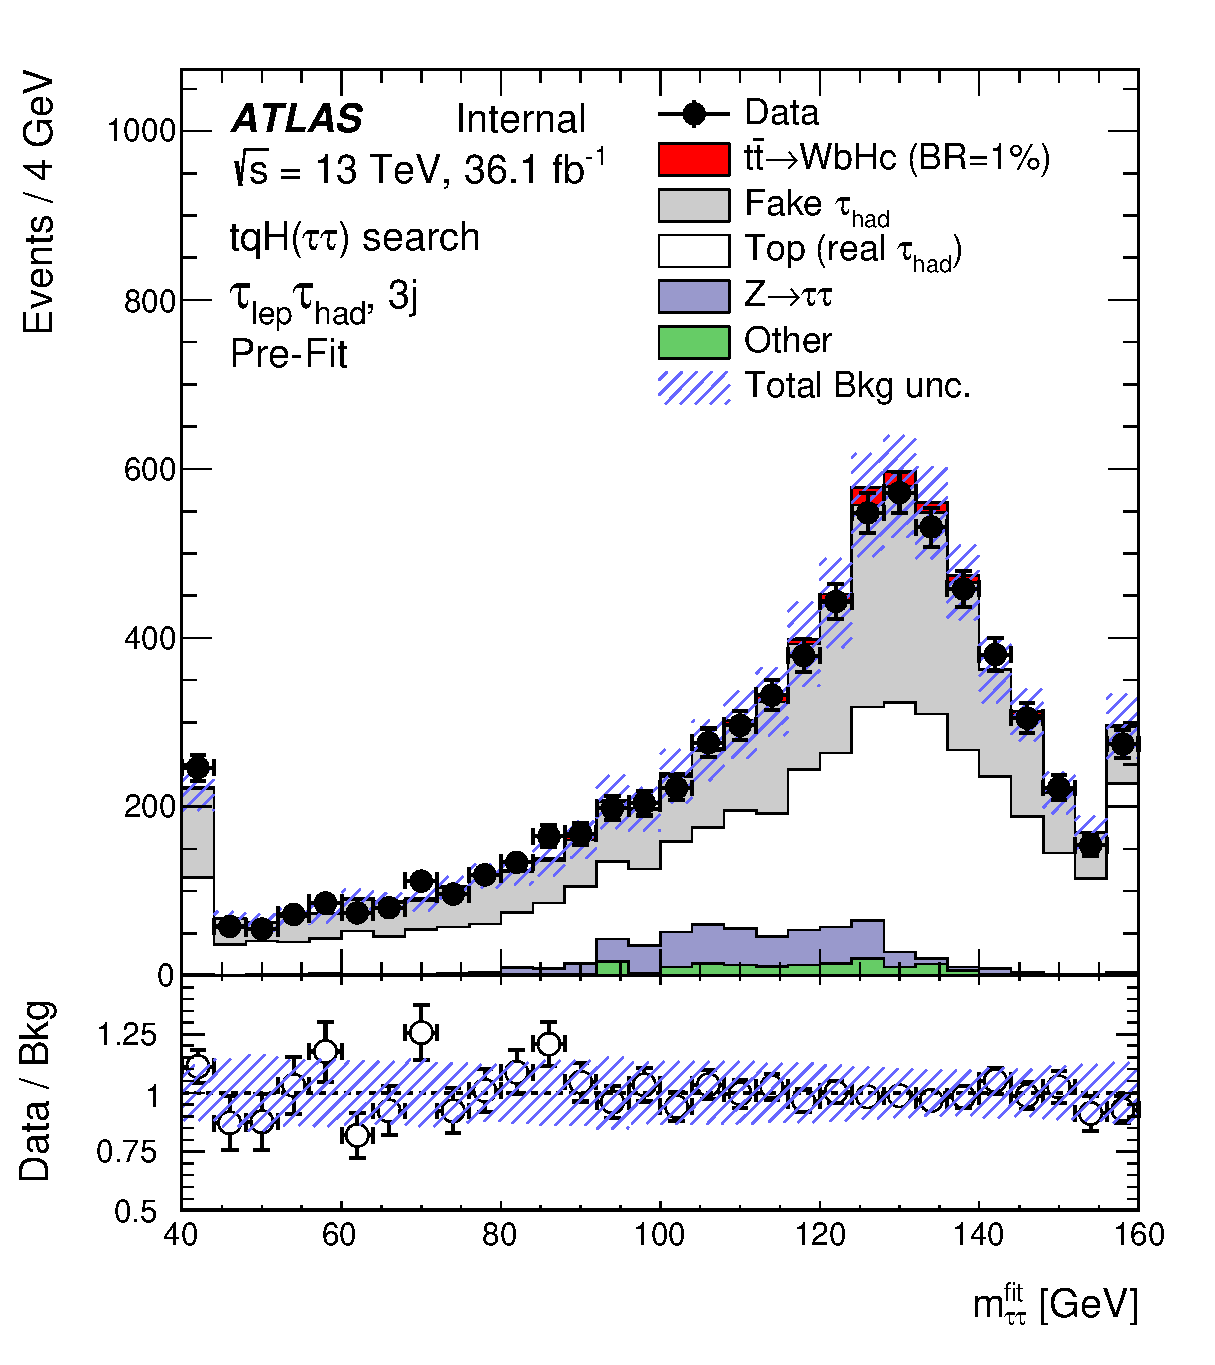
\includegraphics[width=0.40\textwidth]{figures/Htautau/control_plots/m_tt_lephad_3j_FR.eps}}
\subfloat[]{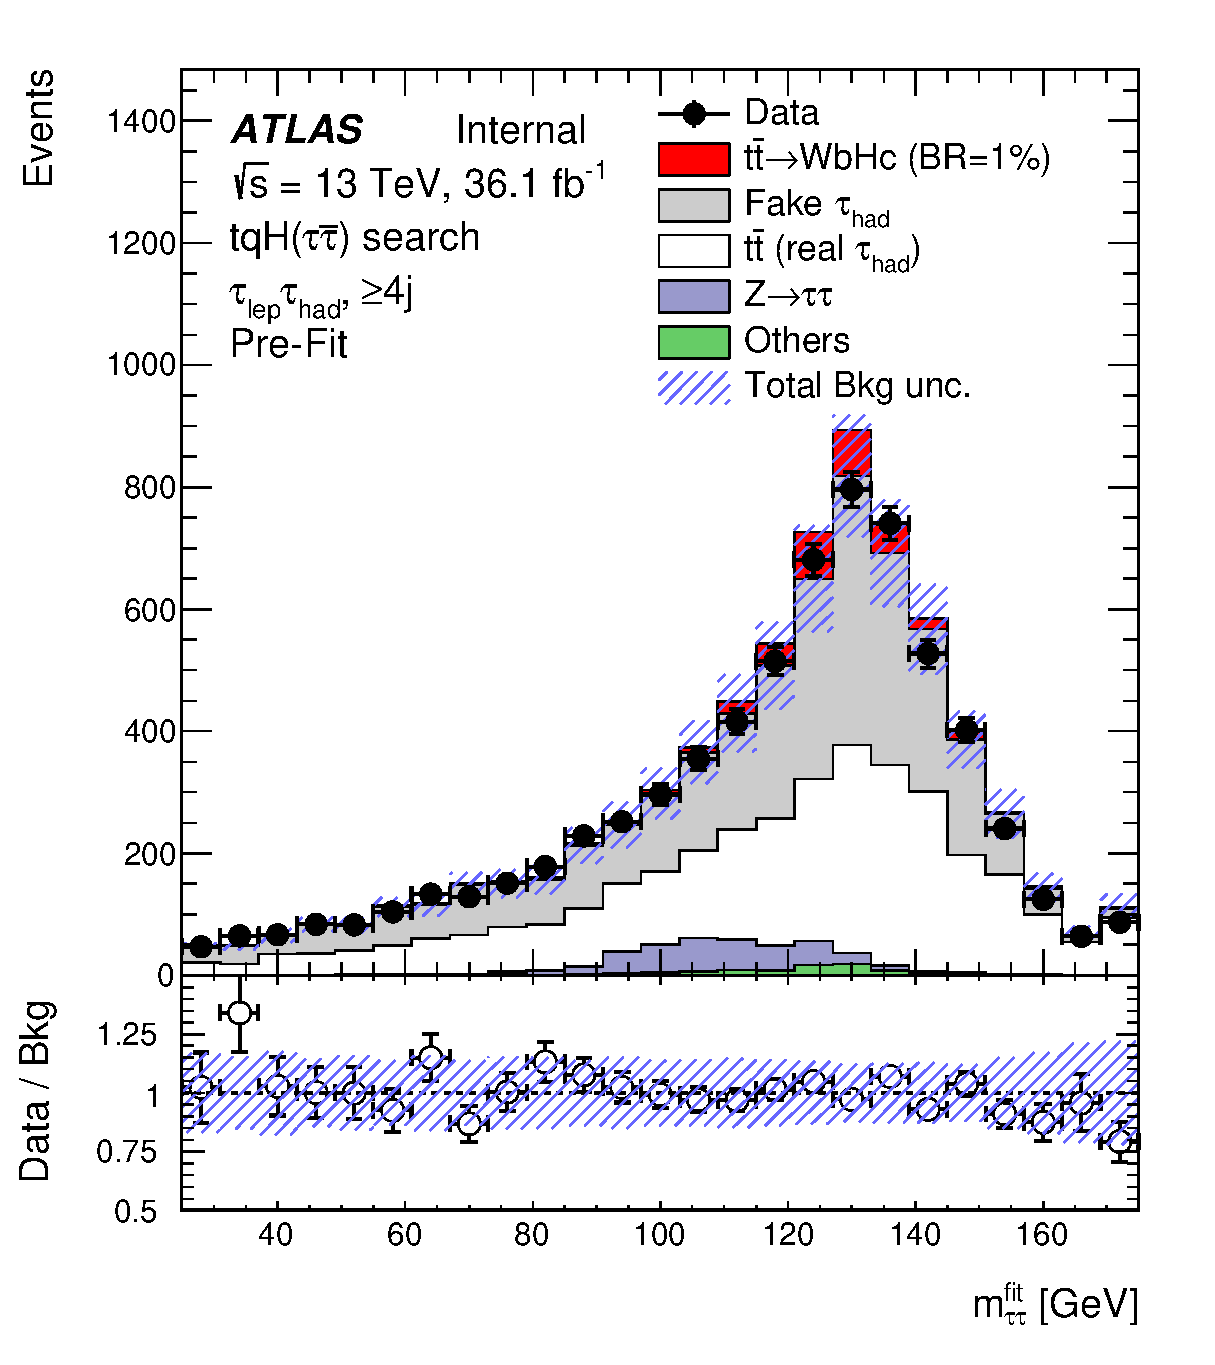
\includegraphics[width=0.40\textwidth]{figures/Htautau/control_plots/m_tt_lephad_4j_FR.eps}} \\
\subfloat[]{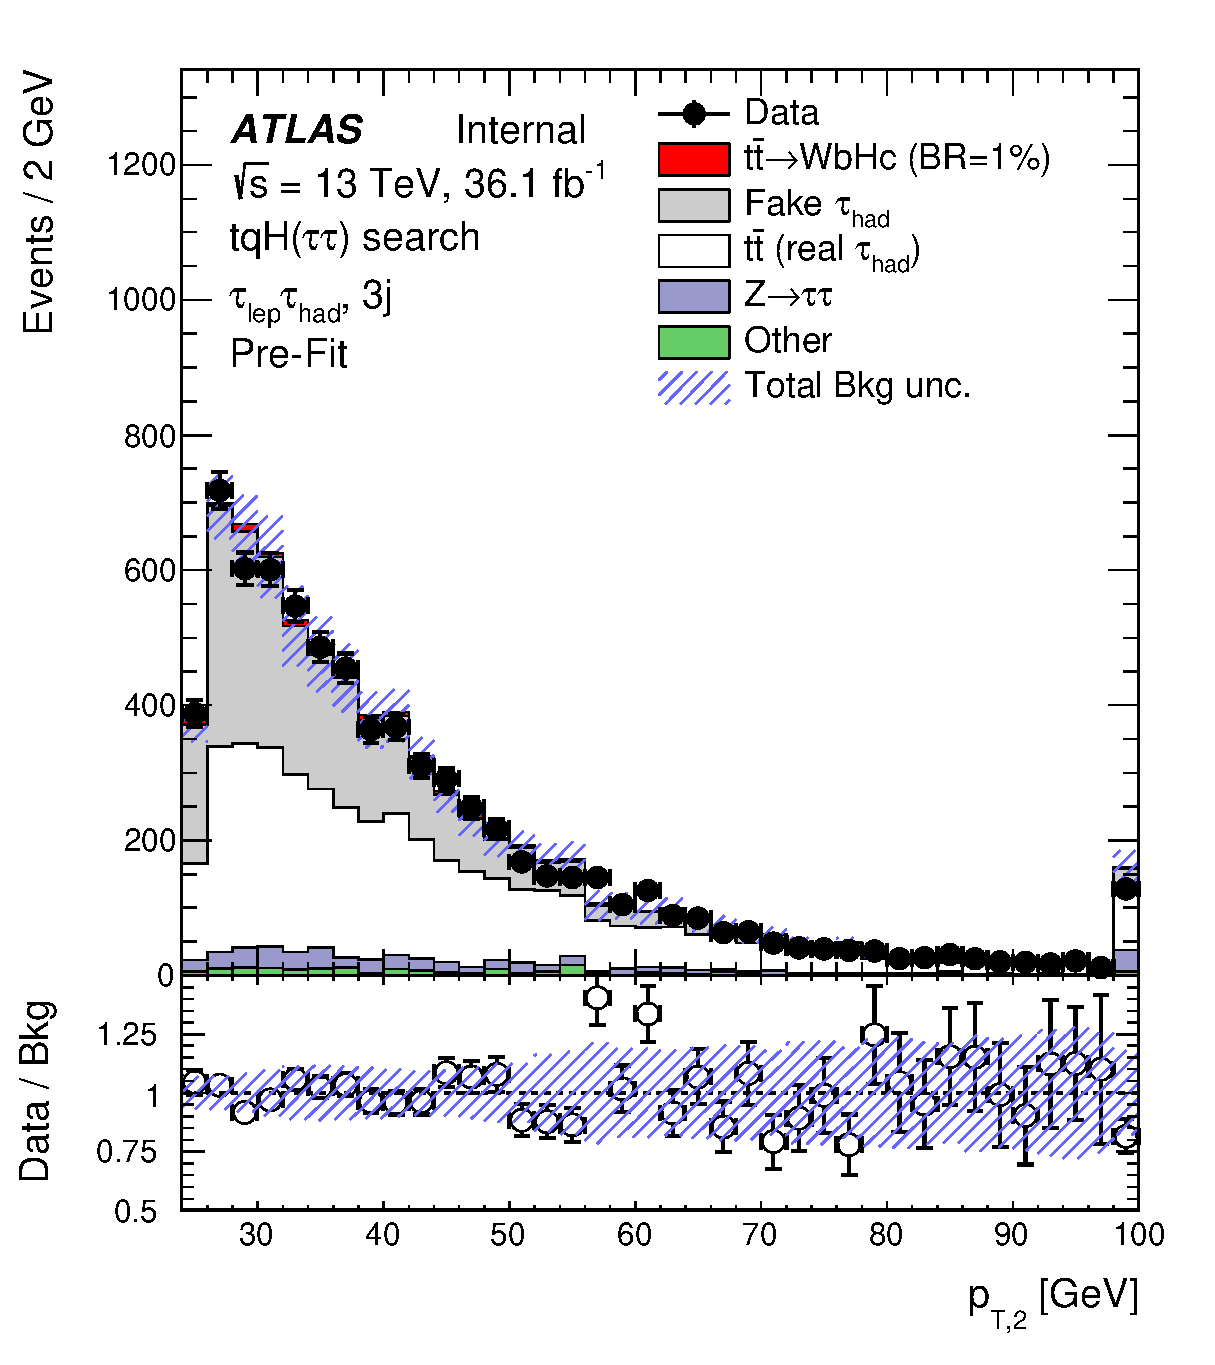
\includegraphics[width=0.40\textwidth]{figures/Htautau/control_plots/ptL2_lephad_3j_FR.eps}}
\subfloat[]{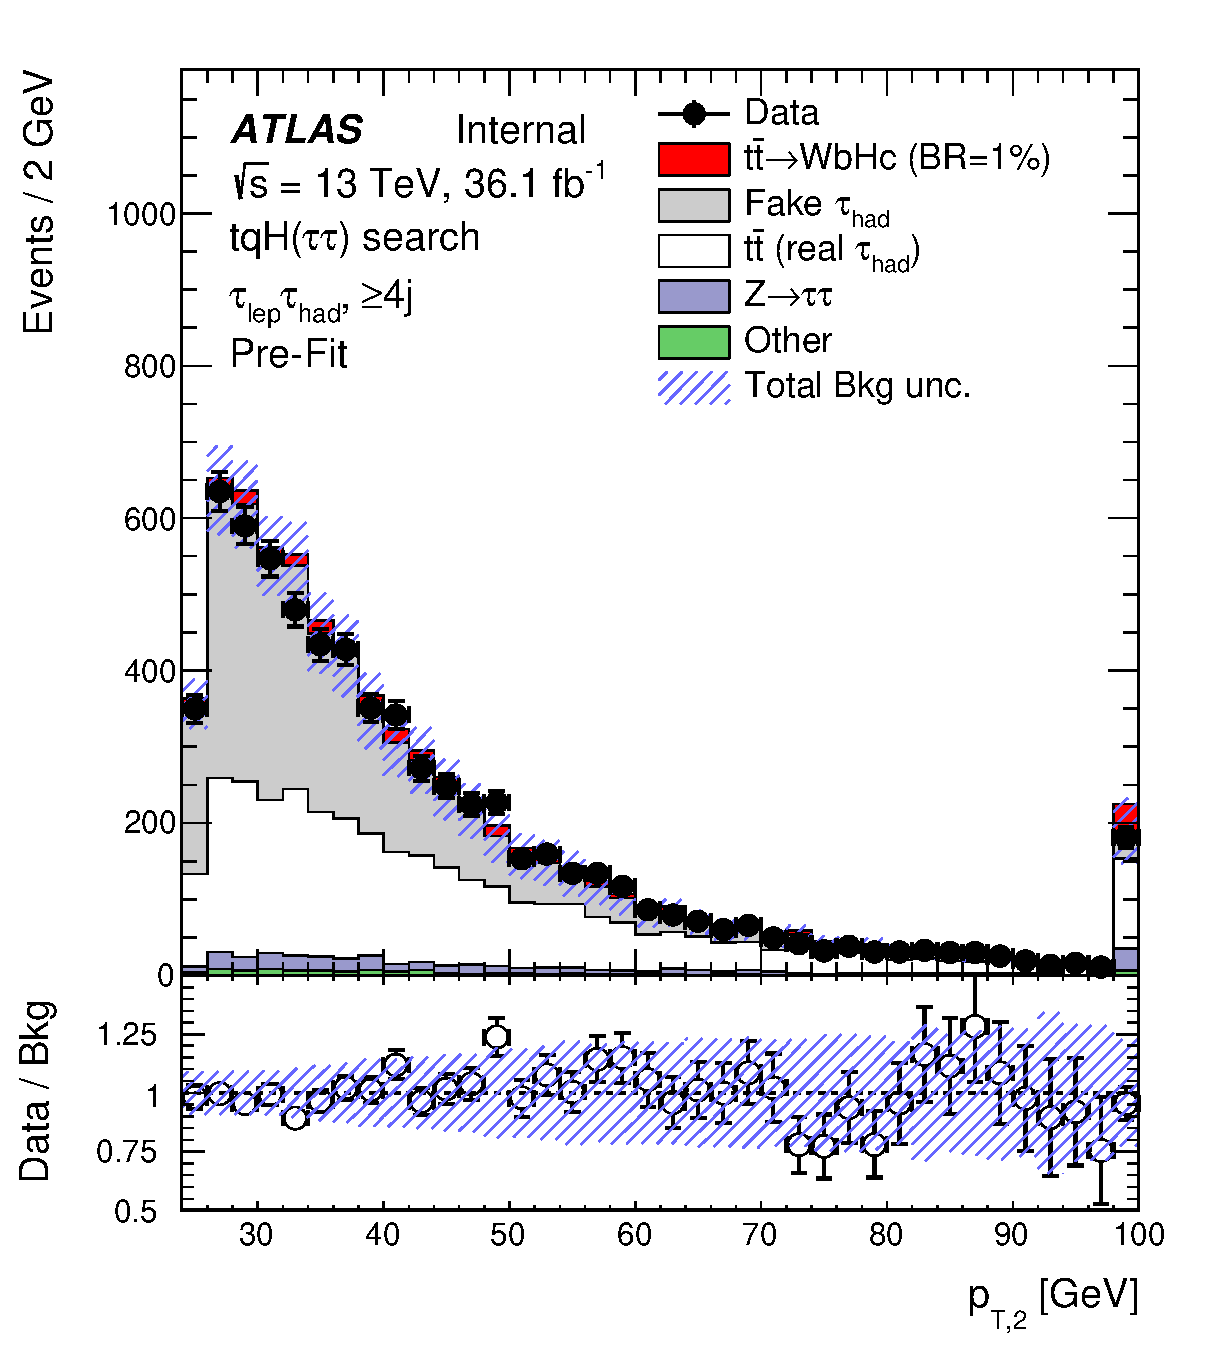
\includegraphics[width=0.40\textwidth]{figures/Htautau/control_plots/ptL2_lephad_4j_FR.eps}} \\
\caption{$\Htautau$ search: Comparison between the data and background prediction for the distribution of some of the most
important BDT input variables in the $\lephad$ channel before performing the fit to data (``Pre-Fit''). The distributions are shown for
$m_{\tau\tau}^{\text{fit}}$ in (a) the ($\lephad$, 3j) region and (b) the ($\lephad$, $\geq$4j) region, and for
$p_{\text{T},2}$ in (c) the ($\lephad$, 3j)  region and (d) the ($\lephad$, $\geq$4j) region.
The contributions with real $\tauhad$ candidates from $\ttbar$,  $\ttbar V$, $\ttbar H$, and single top backgrounds are combined into
a single background source referred to as ``Top (real $\tauhad$)", whereas the small contributions from 
$Z\to \ell^+\ell^-$ ($\ell = e, \mu$) and diboson backgrounds are combined into ``Other''. 
The expected $\Hc$ signal (solid red) corresponding to $\BR(t\to Hc)=1\%$ is also shown,
added on top of the background prediction.
The last bin in all figures contains the overflow.
The bottom panel displays the ratio of data to the SM background (``Bkg'') prediction. 
The hashed area represents the total uncertainty of the background.}
\label{fig:BDT_inputs_lephad}
\end{center}
\end{figure*}
%%%%%%%%%%%%%%%%%%%%%%%%%%%%%%%%%%%%%%%

%%%%%%%%%%%%%%%%%%%%%%%%%%%%%%%%%%%%%%%
\begin{figure*}[t]
\begin{center}
\subfloat[]{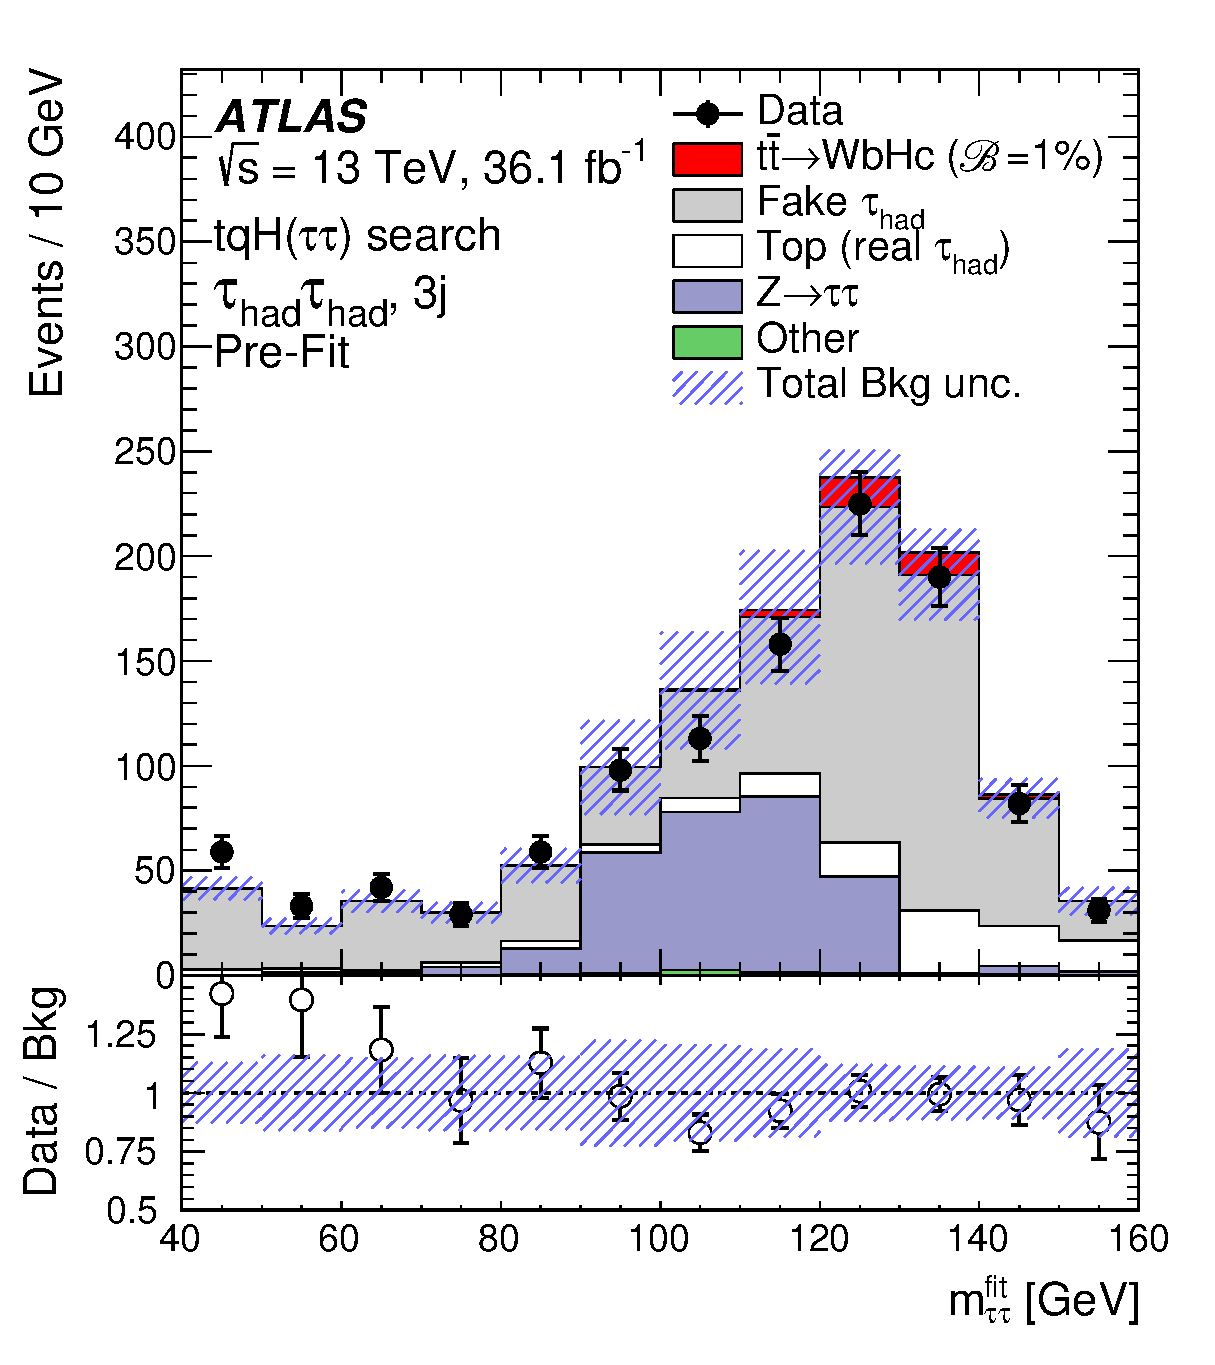
\includegraphics[width=0.40\textwidth]{figures/Htautau/control_plots/m_tt_hadhad_3j_FR.eps}}
\subfloat[]{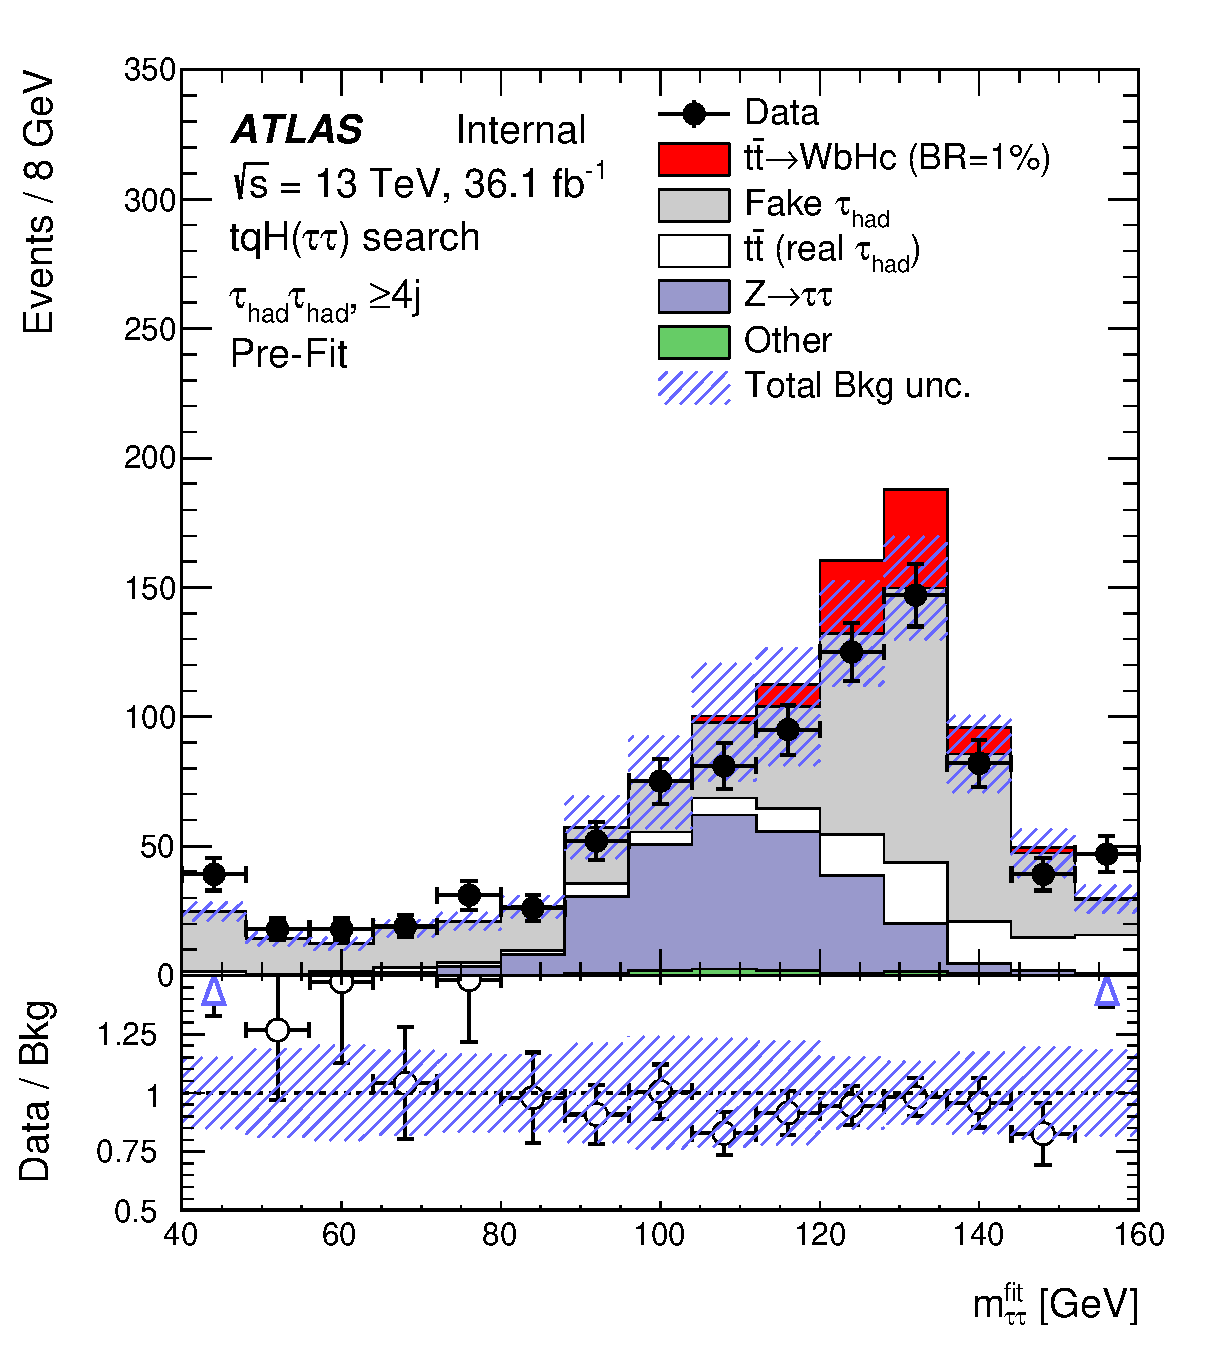
\includegraphics[width=0.40\textwidth]{figures/Htautau/control_plots/m_tt_hadhad_4j_FR.eps}} \\
\subfloat[]{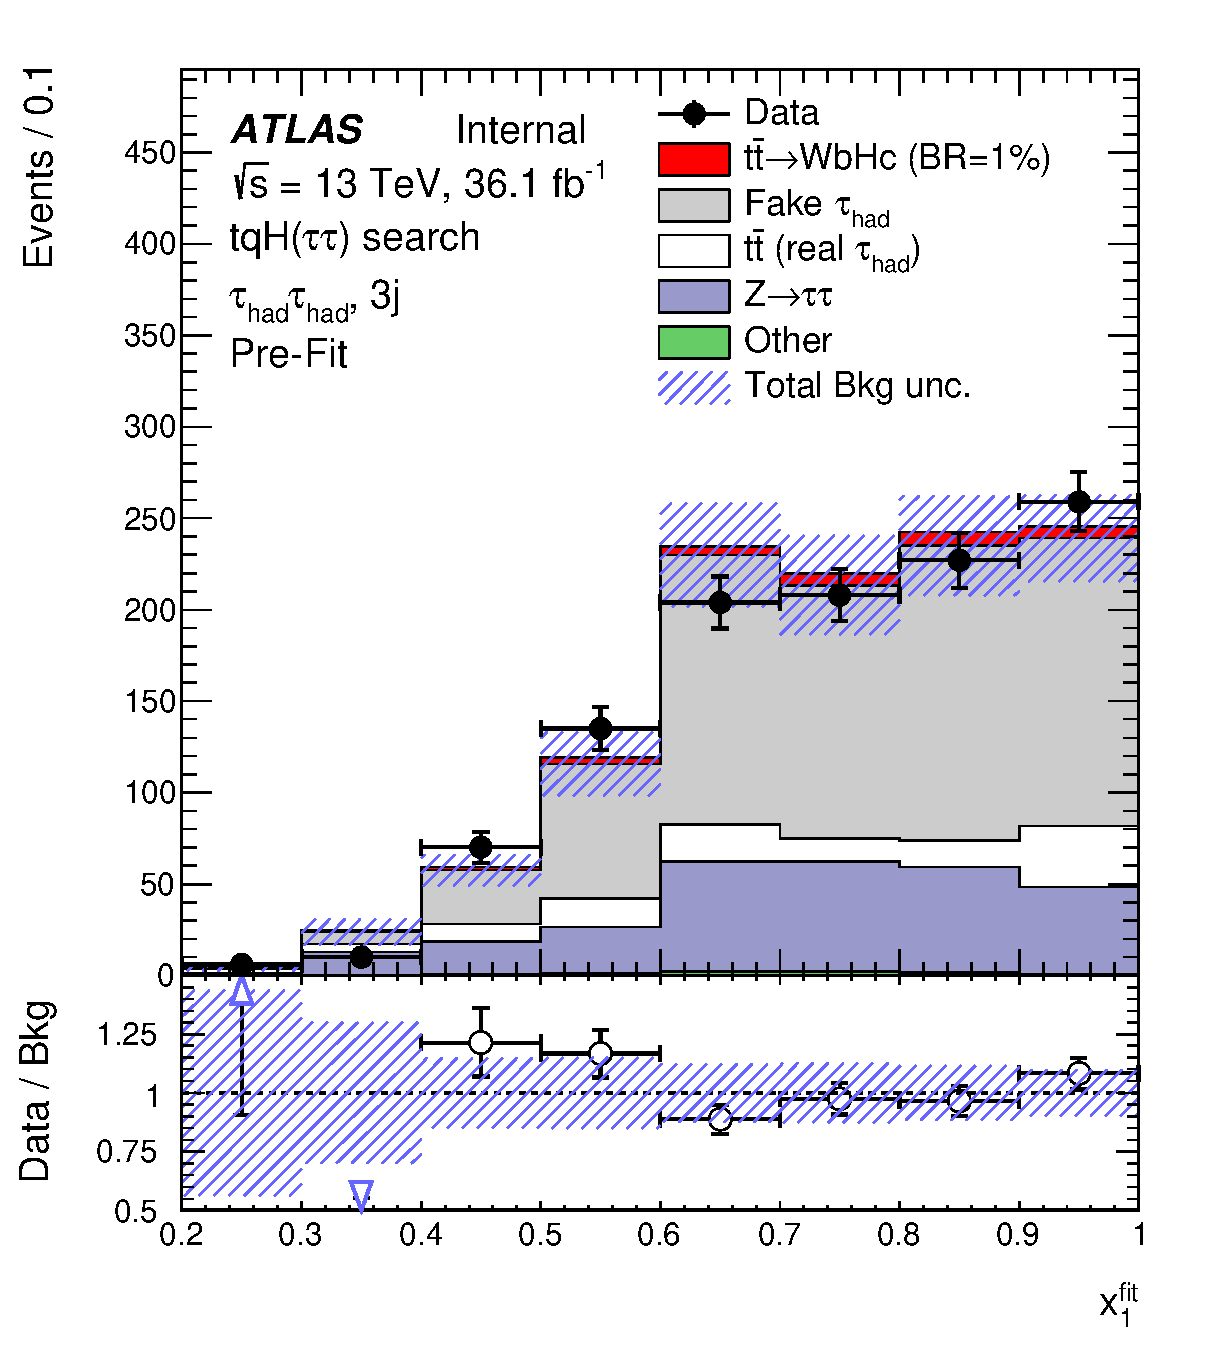
\includegraphics[width=0.40\textwidth]{figures/Htautau/control_plots/x1_fit_hadhad_3j_FR.eps}}
\subfloat[]{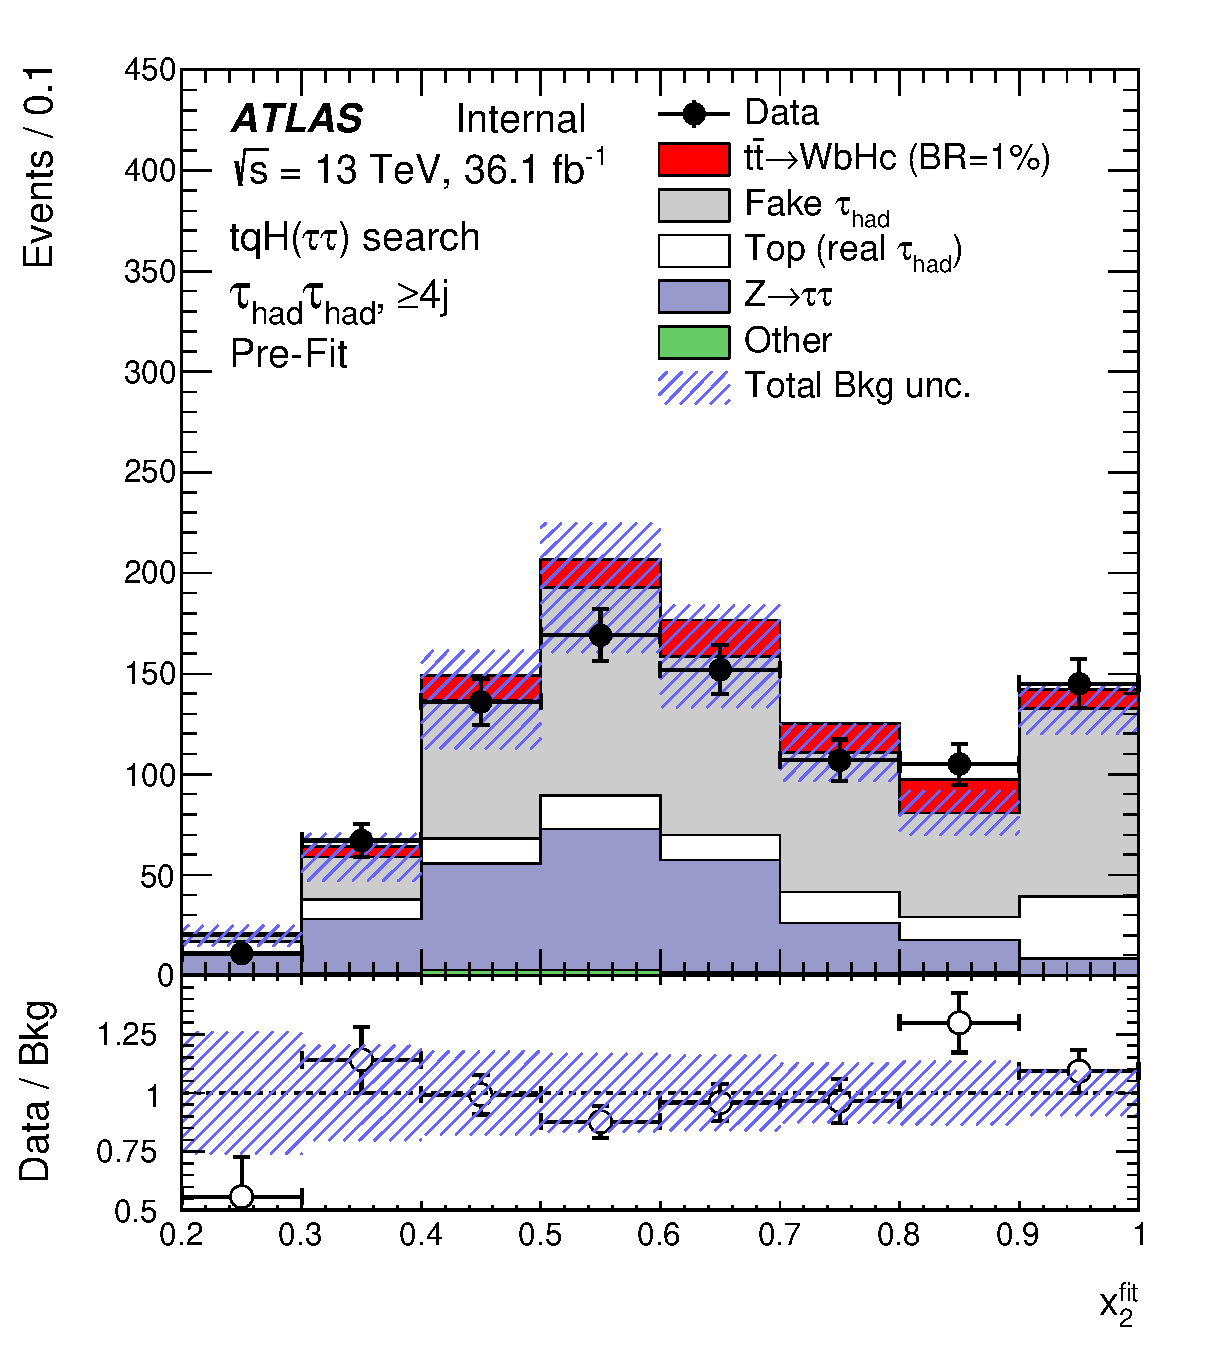
\includegraphics[width=0.40\textwidth]{figures/Htautau/control_plots/x2_fit_hadhad_4j_FR.eps}} \\
\caption{$\Htautau$ search: Comparison between the data and background prediction for the distribution of two of the most 
important BDT input variables in the $\hadhad$ channel before performing the fit to data (``Pre-Fit''). The distributions are shown for
$m_{\tau\tau}^{\text{fit}}$ in (a) the ($\hadhad$, 3j) region and (b) the ($\hadhad$, $\geq$4j) region, and for
(c) $x_{1}^{\text{fit}}$ in the ($\hadhad$, 3j)  region, and (d) $x_{2}^{\text{fit}}$ in the ($\hadhad$, $\geq$4j) region.
The contributions with real $\tauhad$ candidates from $\ttbar$,  $\ttbar V$, $\ttbar H$, and single top backgrounds are combined into
a single background source referred to as ``Top (real $\tauhad$)", whereas the small contributions from 
$Z\to \ell^+\ell^-$ ($\ell = e, \mu$) and diboson backgrounds are combined into ``Other''. 
The expected $\Hc$ signal (solid red) corresponding to $\BR(t\to Hc)=1\%$ is also shown,
added on top of the background prediction.
The last bin in all figures contains the overflow.
The bottom panel displays the ratio of data to the SM background (``Bkg'') prediction. 
The blue triangles indicate points that are outside the vertical range of the figure. 
The hashed area represents the total uncertainty of the background. } 
\label{fig:BDT_inputs_hadhad}
\end{center}
\end{figure*}
%%%%%%%%%%%%%%%%%%%%%%%%%%%%%%%%%%%%%%%

%%%%%%%%%%%%%%%%%%%%%%%%%%%%%%%%%%%%%%%
\begin{figure*}[t]
\begin{center}
\subfloat[]{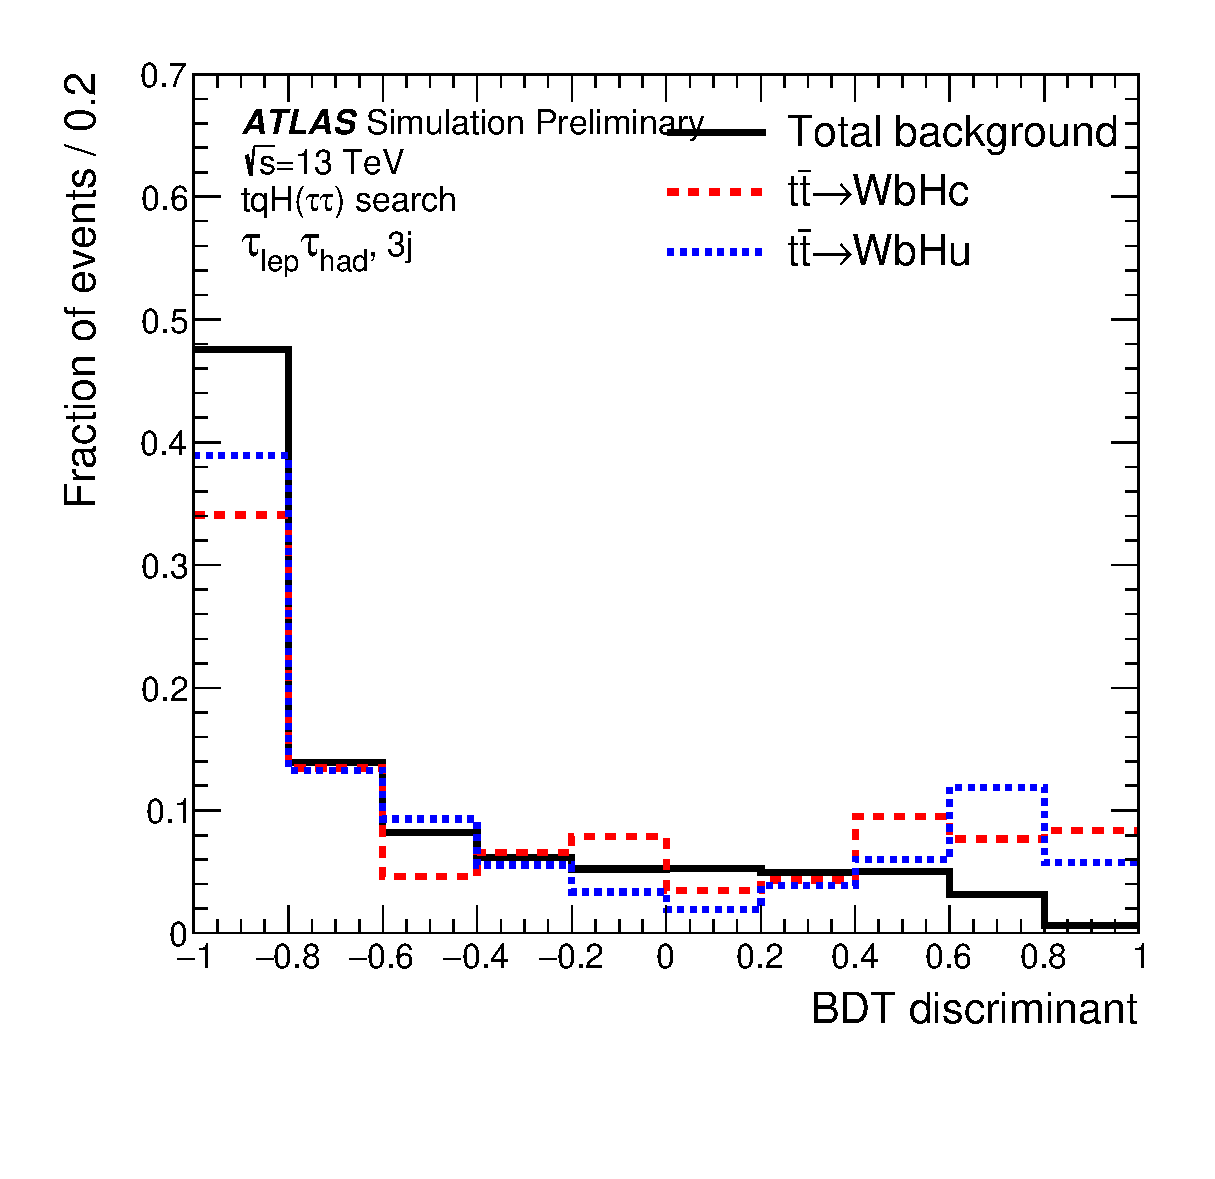
\includegraphics[width=0.40\textwidth]{figures/Htautau/discriminant_shape/shape_discriminant_hl3j/canv_.eps}}
\subfloat[]{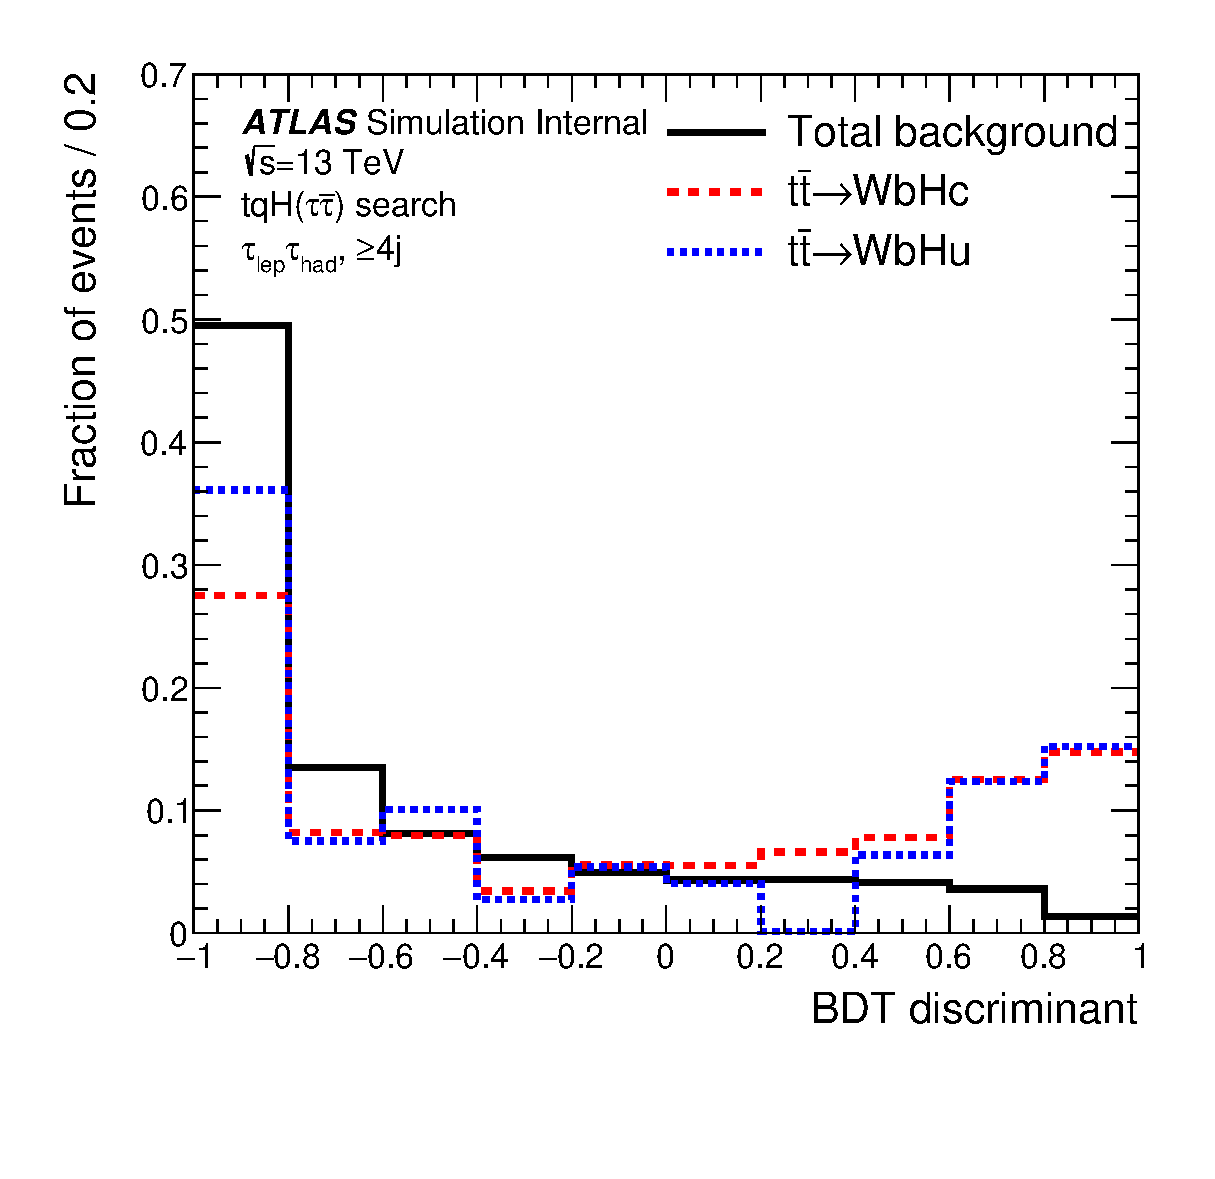
\includegraphics[width=0.40\textwidth]{figures/Htautau/discriminant_shape/shape_discriminant_hl4j/canv_.eps}} \\
\subfloat[]{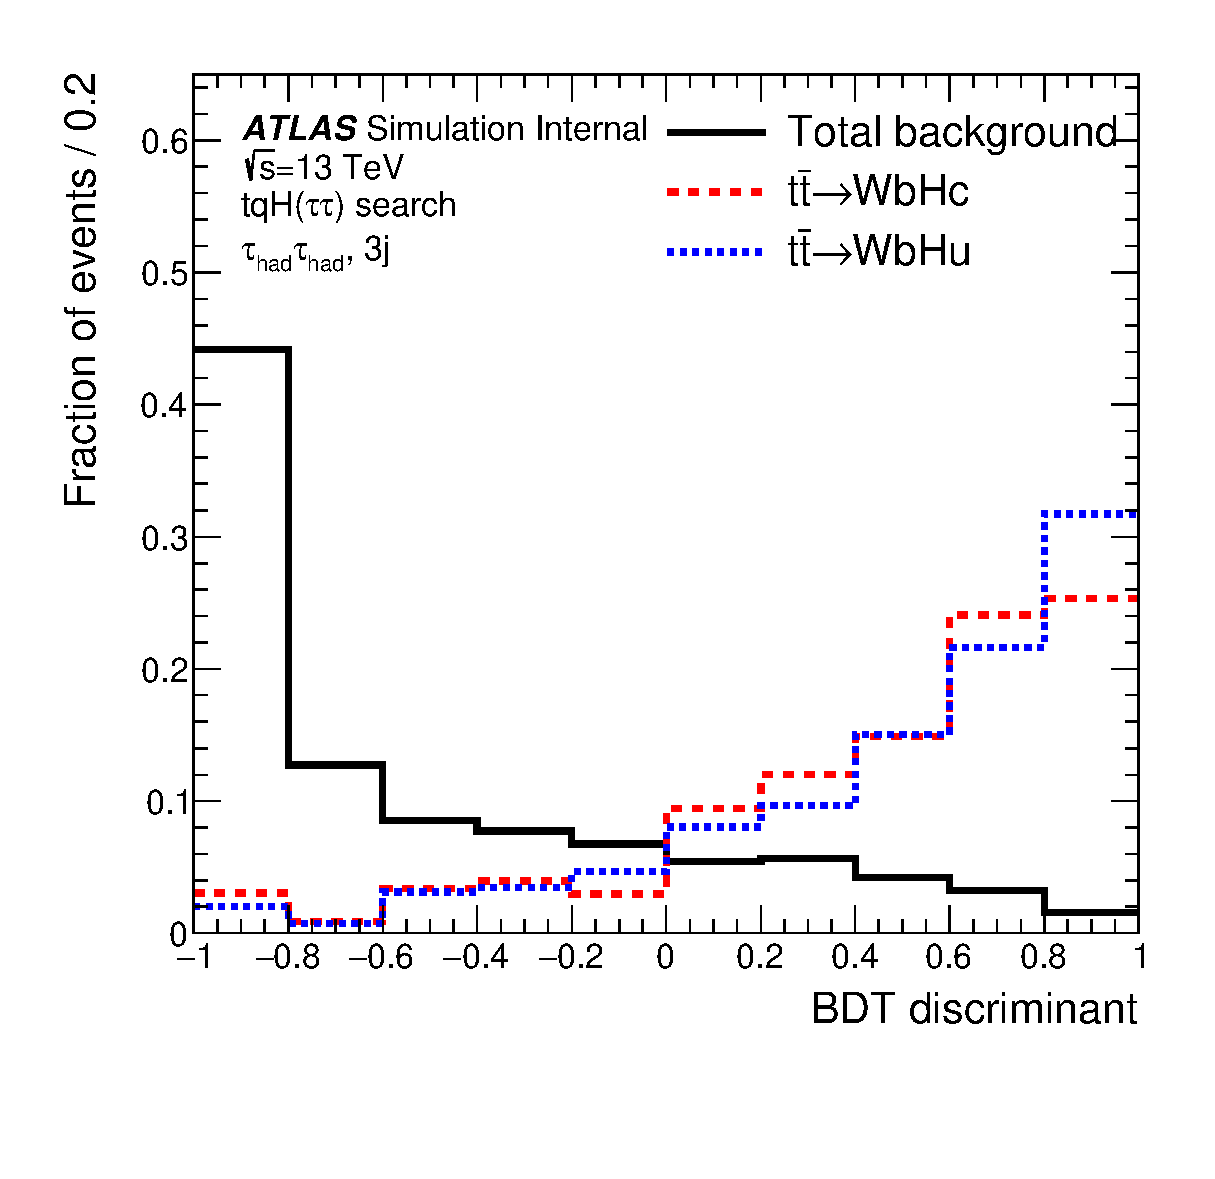
\includegraphics[width=0.40\textwidth]{figures/Htautau/discriminant_shape/shape_discriminant_hh3j/canv_.eps}}
\subfloat[]{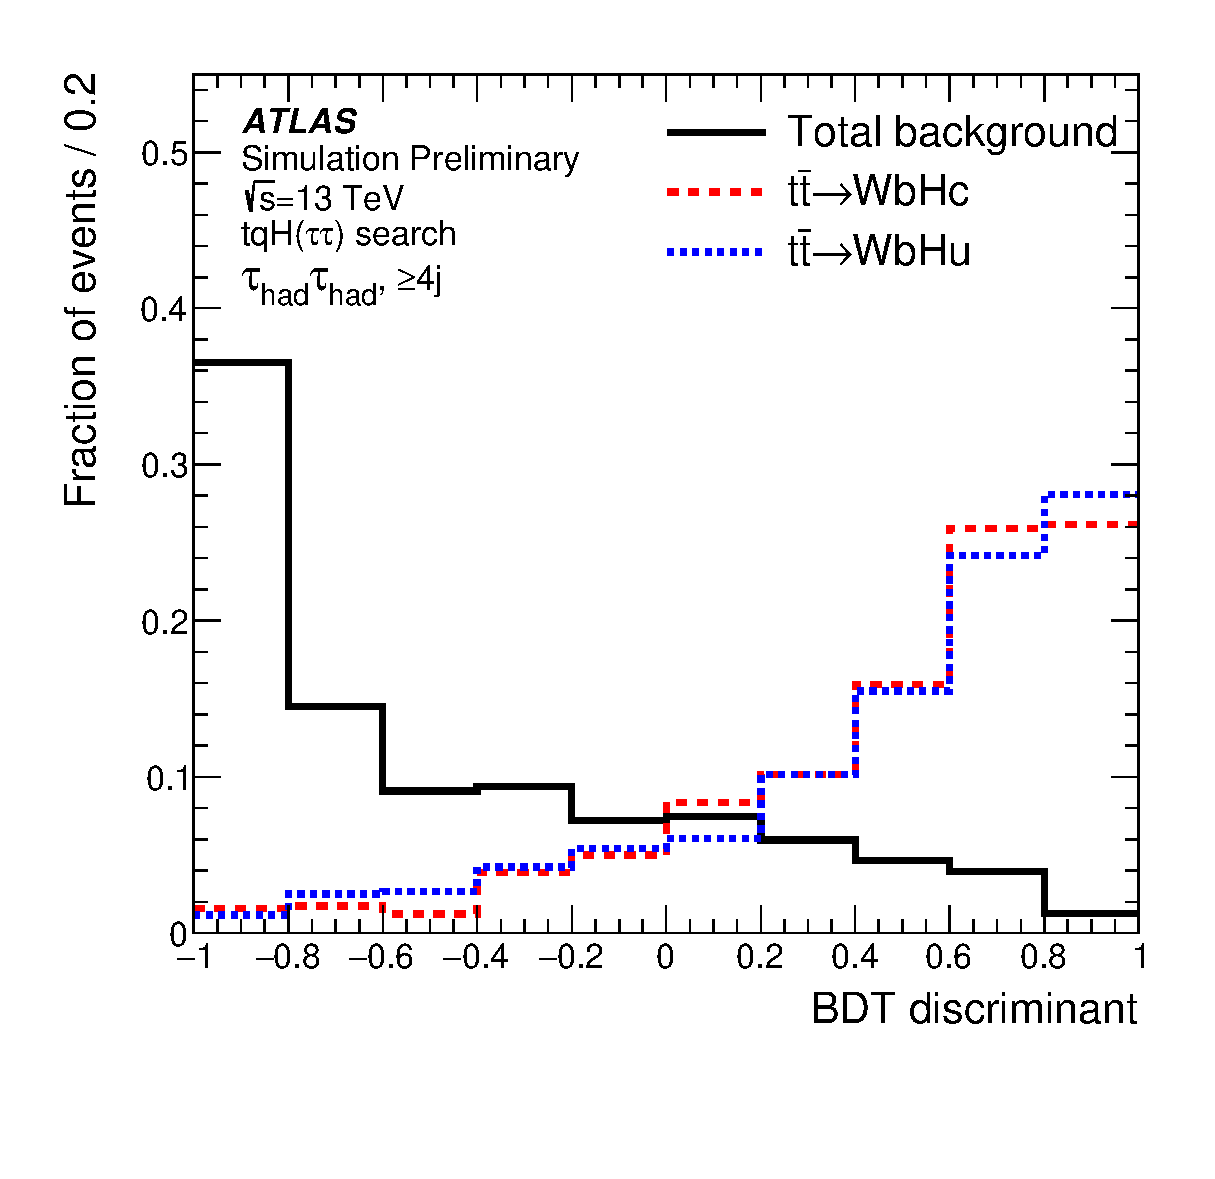
\includegraphics[width=0.40\textwidth]{figures/Htautau/discriminant_shape/shape_discriminant_hh4j/canv_.eps}} \\
\caption{$\Htautau$ search: Comparison of the shape of the BDT discriminant distribution between the $\Hc$ (red dashed) and $\Hu$ (blue dotted) signals, 
and the total background (black solid) in the different search regions considered:
(a) ($\lephad$, 3j), (b) ($\lephad$, $\geq$4j), (c) ($\hadhad$, 3j), and (d) ($\hadhad$, $\geq$4j). }
\label{fig:BDT}
\end{center}
\end{figure*}
%%%%%%%%%%%%%%%%%%%%%%%%%%%%%%%%%%%%%%%%%%%%%%%%%% 
